\documentclass[11pt, oneside]{article}   	% use "amsart" instead of "article" for AMSLaTeX format
\usepackage{geometry}                		% See geometry.pdf to learn the layout options. There are lots.
\geometry{letterpaper}                   		% ... or a4paper or a5paper or ... 
%\geometry{landscape}                		% Activate for rotated page geometry
%\usepackage[parfill]{parskip}    		% Activate to begin paragraphs with an empty line rather than an indent
\usepackage{graphicx}				% Use pdf, png, jpg, or eps§ with pdflatex; use eps in DVI mode
\usepackage{amsmath}								% TeX will automatically convert eps --> pdf in pdflatex		
\usepackage{amssymb}


\title{Determining Initial Conditions Required for a Projectile Based Commute}
\author{David Abramov}	

\begin{document}
\maketitle
\section{The Problem}

Becoming a projectile is a great way to save time on your daily commute as well as eliminate stressors associated with the unpredictable nature of public transportation or interactions with terrible drivers. Before becoming a projectile, it is crucial to know what your initial velocity vector must be in order to land at your desired destination. In order to do this, the distance between your starting point and destination must be known, as well as the height of your destination versus your starting point. From there, a launch angle $\theta$ and initial speed $v_{0}$ can be chosen and tested mathematically before subjecting oneself to a potentially fatal flightpath.

\section{Known and Unknown Quantities}

Table 1 shows the known and unknown quantities for this problem. East is the +$x$ direction and North is in the +$y$. Byrne Hall is about 800 meters East of my apartment, and 2100 meters South. The linear distance between my apartment and Byrne Hall, $\Delta d$, is about 2247 meters, calculated using the Pythagorean theorem. The height of Byrne Hall, $h_{Byrne}$, is approximately 18 meters. The gravitational constant, $g$, will also be of use, and has a value of 9.80665 m/s$^2$. The unknown quantities are the initial velocity vector, $\vec{v}_{0}$, the launch angle relative to the ground, $\theta$, the total time of the flight, $t_{total}$, the maximum height of the flight, $h_{max}$, and the $z$ component of the velocity vector, $v_{z}$.

\begin{table}[h!]
\centering
\begin{tabular}{||c | c||} 
 \hline
 Known Quantities & Unknown Quantities \\ [0.5ex] 
 \hline\hline
 $x = 800$ m & $\vec{v}_{0}$ \\ 
 $y = -2100$ m &  $\theta$  \\
 $\Delta d$ = 2247 m & $t_{total}$ \\ 
 $h_{Byrne}$ = 18 m & $h_{max}$\\ 
 $g$ = 9.80665 m/s$^2$& $v_{z}$ \\[1ex] 
 \hline
\end{tabular}
\caption{Known and Unknown Quantities}
\label{table:1}
\end{table}

\vphantom{1}

\section{Drawing}
Figure 1 shows the relative distance between my apartment and Byrne Hall. Distances were acquired using Google Maps.
\begin{figure}
\centering
  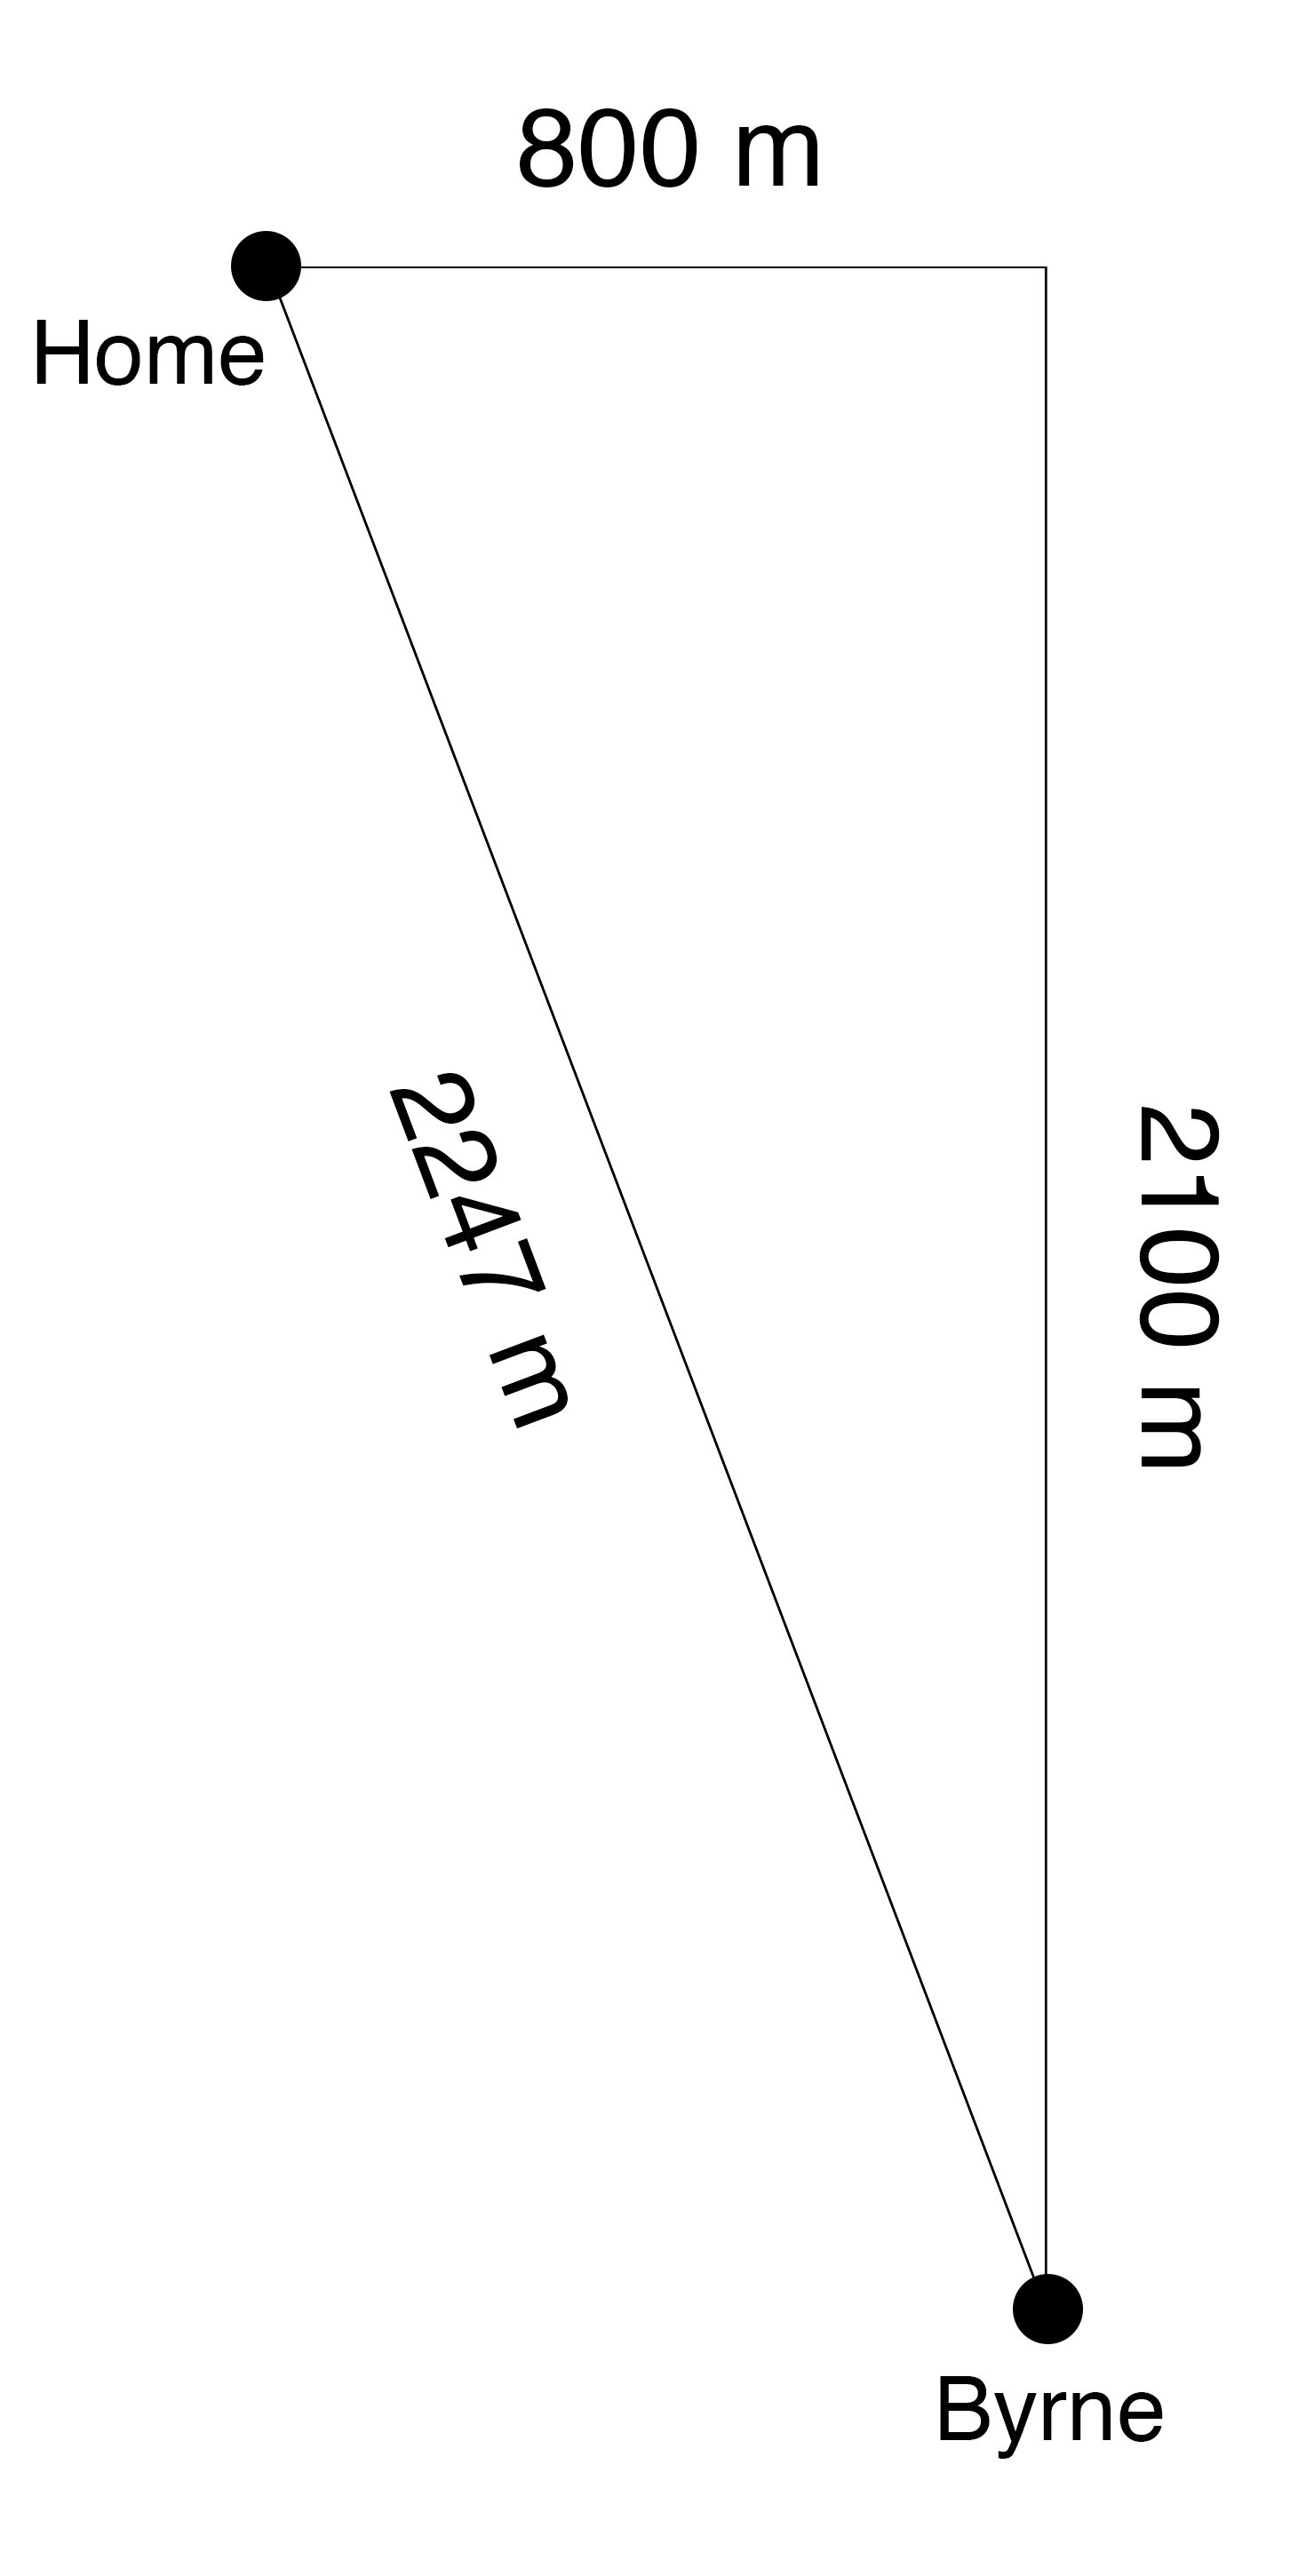
\includegraphics[width=100px]{location.jpg}
  \caption{Relative distance between home and Byrne Hall.}
  \label{fig:boat1}
\end{figure}

\section{Steps and Approach}

Given an initial velocity and launch angle, Equations (1) can be used to determine the distance traveled horizontally,

\begin{equation}
d=v_{0}t\cos\theta
\end{equation}

\noindent and (2) can be used to find the vertical position at a particular time.

\begin{equation}
h=v_{0}t\sin\theta - \frac{1}{2}gt^2
\end{equation}

\noindent Because the vertical position is dependent on the gravitational constant, $g$, and the equation for the horizontal position does not, Eq. (3) can be used to find the total time duration of a flight by setting $h$ to 18 meters, and solving for $t$.

\begin{equation}
0=\frac{1}{2}gt^2 - v_{0}t\sin\theta  + 18
\end{equation}

\noindent Equation (4) gives the total for the length of the flight, $t$, for an initial velocity, $v_{0}$, and launch angle, $\theta$.
\begin{equation}
t_{total} = -\frac{v_{0}\sin\theta\pm\sqrt{v_{0}^2\sin^2\theta-36g}}{g}
\end{equation}

\noindent In order to find the maximum height $\frac{t}{2}$ can be plugged in for $t$ in Eq. (2), however this also means that Eq. (2) must be solved for $t$ when $h = 0$, which is given by Eq. (5).

\begin{equation}
t_{h,max} = \frac{1}{2} \frac{v_{0}\sin\theta\pm\sqrt{v_{0}^2\sin^2\theta}}{g}
\end{equation}

\noindent Equation (6) gives the maximum height of the projectile when $t = t_{h,max}$.
\begin{equation}
h_{max} = \frac{1}{2}v_{0}t_{h,max}\sin\theta-\frac{1}{8}gt_{h,max}^2
\end{equation}

%The horizontal velocity can be found by dividing $\Delta d$ by $t_{total}$.
%
%\begin{equation}
%v_{x} = \frac{\Delta d}{t_{total}}
%\end{equation}

%\noindent Equation (7) gives the initial velocity vector $\vec{v}_{0}$ in cartesian coordinates. The components $v_{x}$ and $v_{y}$ are known, where $+v_{x}$ corresponds to Byrne Hall being east of my apartment, and $-v_{y}$ corresponds to Byrne being south. The $v_{z}$ component is unknown. Each component is divided by $t_{total}$ to give the proper units of $\frac{m}{s}$.
%\begin{equation}
%%\vec{v}_{0}= \frac{1}{t_{total}}[800\hat{x}-2100\hat{y}+v_{z}\hat{z}]
%\vec{r}= (800\textnormal{ m})\hat{x}-(2100\textnormal{ m})\hat{y}+(18\textnormal{ m})\hat{z}
%\end{equation}


%\noindent Equation (8) gives the magnitude of $\vec{v}_{0}$ as the the square root of the sum of the squares of each of the components,
%
%\begin{equation}
%|\vec{v_{0}}| = \frac{1}{t}\sqrt{800^2+2100^2+v_{z}^2}
%\end{equation}
%
%\noindent and can be rearranged to find and equation for $v_{z}$ in Eq. (9).
%
%\begin{equation}
%v_{z} = \sqrt{t^2v_{0}^2-800000}
%\end{equation}

\section{Limiting and Special Cases}

Realistically, the angle of the initial velocity vector, $\theta$, must be less than $90^{\circ}$ and greater than $0^{\circ}$, however for very small angles the equations of motion begin to break down. The hypothetical minimum angle, hypothetical because you would have to be launched at an infinite speed, can be found by creating a right triangle where the base is the distance $\Delta d$ between the destination and the starting point (2247 meters in this case), the height of the triangle would be the landing height (in this case 18 meters), and the angle $\theta$ can be found by by taking $\tan^{-1}(\frac{h}{\Delta d})$.

\begin{equation}
\theta = \tan^{-1}(\frac{18}{2247}) = 0.46^{\circ}
\end{equation}

The magnitude of $\vec{v}_{0}$ that will work is dependent on the angle $\theta$ that is chosen. For example, if $\theta$ is very small, then a very large initial speed would be required to ensure that the desired destination is reached.

\section{Order of Magnitude of Numerical Answers}\

Because many different initial velocity vectors, $\vec{v_{0}}$, would work, a specific case can be used to give an example of a resulting trajectory. If a launch angle of $\theta = 45^{\circ}$ is chosen as well as an initial velocity of $|\vec{v_{0}}| = 40$ m/s, these values can be plugged into Eq. (4) to find the total length of the flight.

\begin{equation}
t_{total} = -\frac{40\sin(45^{\circ})\pm\sqrt{40^2\sin^{2}(45^{\circ})-36g}}{g} = 6.36 \textnormal{ seconds}
\end{equation}

%\noindent This time can now be used to find the component $v_{z}$, and subsequently the initial velocity vector $\vec{v}_{0}$.
%
%\begin{equation}
%v_{z} = \sqrt{(6.36\textnormal{ s})^{2}(40\textnormal{ m/s})^2-800000} = 2526 \textnormal{ meters}
%\end{equation}

%\noindent Plugging this back into Eq. (7), which gives the initial velocity vector $\vec{v}_{0}$ in cartesian coordinates,
%
%\begin{equation}
%\vec{v}_{0}= \frac{1}{6.36 \textnormal{ s}}[(800 \textnormal{ m})\hat{x}-(2100\textnormal{ m})\hat{y}+(2526\textnormal{ m})\hat{z}]
%\end{equation}
%
%The magnitude of the initial velocity vector, $|\vec{v_{0}}|$, can now be found as well.
%
%\begin{equation}
%|\vec{v_{0}}| = \frac{1}{6.36}\sqrt{800^2+2100^2+2526^2} = 532 \textnormal{ m/s}
%\end{equation}

The time at which the maximum height is reached can be found using Eq. (5).

\begin{equation}
t_{h,max} = \frac{1}{2} \frac{40\sin(45^{\circ})\pm\sqrt{{40}^2\sin^{2}(45^{\circ})}}{g} = 3.47 \textnormal{ seconds}
\end{equation}

This can now be used to find the maximum height of the trajectory.

\begin{equation}
h_{max} = \frac{1}{2}(40 \textnormal{ m/s})(3.47 \textnormal{ s})\sin(45^{\circ})-\frac{1}{8}g (3.47 \textnormal{ s})^2 = 59.1 \textnormal{ meters}
\end{equation}

The horizontal velocity can be found by dividing the total horizontal distance by the total amount of time.

\begin{equation}
v = \frac{\Delta d}{t_{total}} = \frac{2247 \textnormal{ m}}{6.36 \textnormal{ s}} = 353.3 \textnormal{ m/s}.
\end{equation}

Using this, along with Equation (2), the horizontal and vertical positions of the projectile can be modeled using following equations, where $x$ is the position along the straight path between my apartment and Byrne Hall, and $y$ is the height of the projectile.

\begin{equation}
x = (353.3 \textnormal{ m/s})t
\end{equation} 

\begin{equation}
y = (40 \textnormal{ m/s})\sin(40^{\circ})t-0.5gt^2
\end{equation} 

Plugging these values into MatLAB provides the graph shown in Figure 2.

\begin{figure}
\centering
  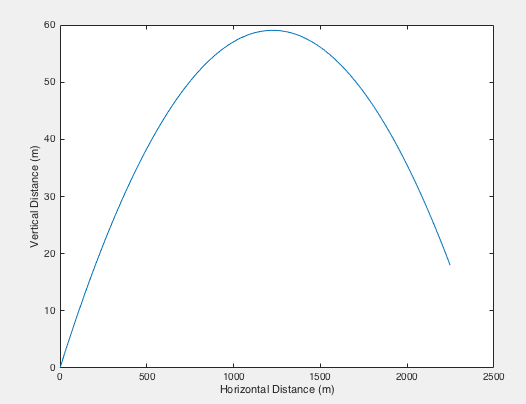
\includegraphics[width=\linewidth]{graph.png}
  \caption{Path of Projectile.}
  \label{fig:boat1}
\end{figure}

\section{Discussion}

The numerical values found for testing an initial velocity of $|\vec{v_{0}}| = 40$ m/s and a launch angle from the ground of $\theta = 40^{\circ}$ make sense because the total amount of time that the projectile is in the air is determined by Eq. (2). Because the projectile constantly feels the force of gravity, it makes sense that the flight time is on the order of magnitude of several seconds. Because the projectile has to travel a linear distance on the order of several thousand meters, it makes sense that the initial velocity is on the order of several hundred meters per second.

%\subsection{}

\section{Code}

My code is attached as a comment on the D2L dropbox for this assignment.

\end{document}  
